\ylDisplay{Valgusallika kujutis} % Ülesande nimi
{EFO zürii} % Autor
{lahtine} % Voor
{2017} % Aasta
{G 2} % Ülesande nr.
{2} % Raskustase
{
% Teema: Geomeetriline-optika
\ifStatement
Sama suure fookuskauguse absoluutväärtusega $f$ kumer- ja nõguslääts asuvad nii, et nende fookused ning optilised peateljed ühtivad. Läätsede ees optilisel peateljel kumerläätsest kaugusel $\num{1,5}f$ asub punktvalgusallikas $A$. Leidke punktvalgusallika kujutise asukoht läbi kahe läätse. Tehke joonis.
\fi


\ifHint
$A$ asukoha leidmiseks võib kasutada läätsevalemit.
\fi


\ifSolution
Valgusallika kujutist ei tekigi (või tekib lõpmatusse), kuna pärast teise läätse läbimist on valguskiired paralleelsed optilise peateljega.

Valguskiired on paralleelsed, kuna  valgusallika $A$ kujutis läbi kumerläätse tekiks nõgusläätse parempoolsesse fookusesse. Seega kumerläätse läbinud kiired langevad nõgusläätsele nii, et nad koonduksid parempoolses fookuses. Kuna nõguslääts hajutab valgust, siis on kiired pärast nõgusläätse läbimist paralleelsed, mistõttu valgusallika kujutist ei teki (või tekib see lõpmatusse).

\begin{center}
	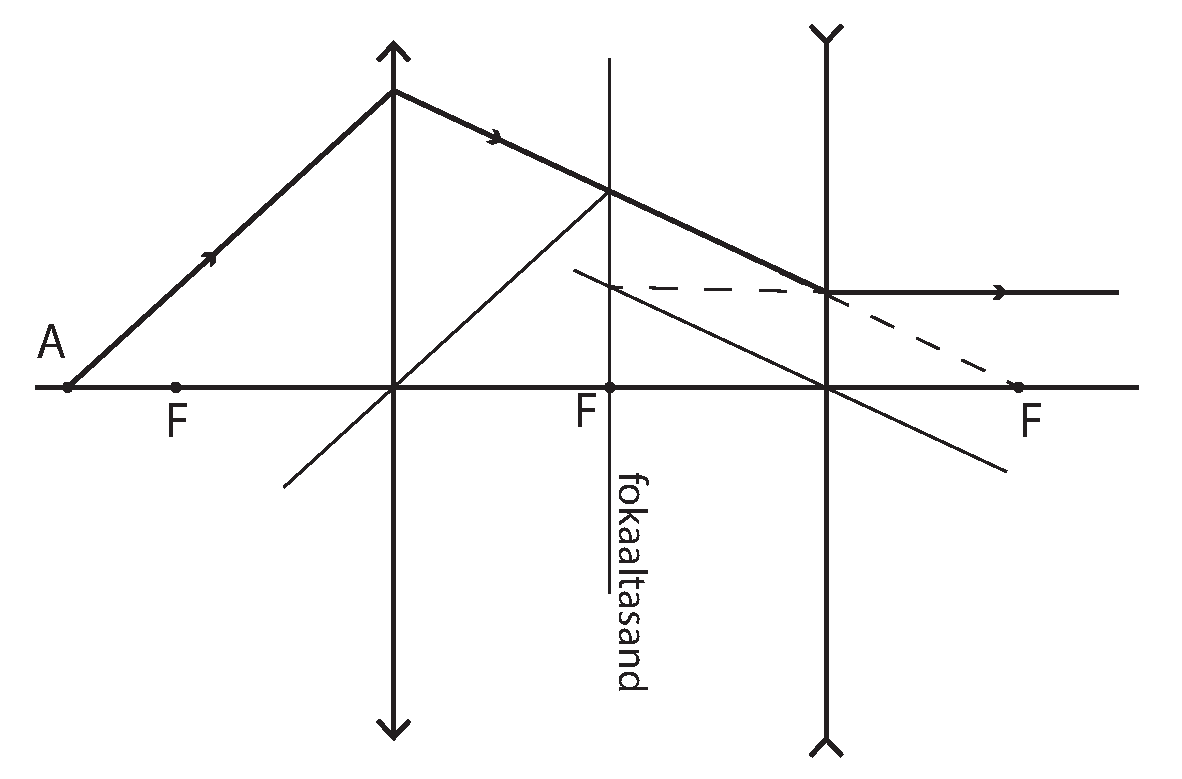
\includegraphics[width=0.7\linewidth]{2017-lahg-02-valgusallikaslah}
\end{center}
\fi


\ifEngStatement
% Problem name: The image of a light source
A concave lens and a convex lens have the same focal length with an absolute value $f$. The lenses are positioned so that their focuses and optical axes coincide. In front of the lenses on the optical axis there is a point light source $A$ at a distance $1,5f$ from the convex lens. Find the location of the point light source's image formed by the two-lens system. Make a draft.
\fi


\ifEngHint
You can use the thin lens formula to find the location of $A$.
\fi


\ifEngSolution
No image of the light source will appear (or it will appear in infinity) because after the light rays have gone through the second lens they are parallel to the optical axis.\\
The light rays are parallel because the image of the light source $A$ through the convex lens would appear in the right focal point of the concave lens. Therefore the rays that went through the convex lens fall on the concave lens so that they would focus in the focal point on the right. Because the concave lens diverges light then the rays are parallel after going through the concave lens which is why no image of the light source will appear (or it will appear in infinity).
\begin{center}
	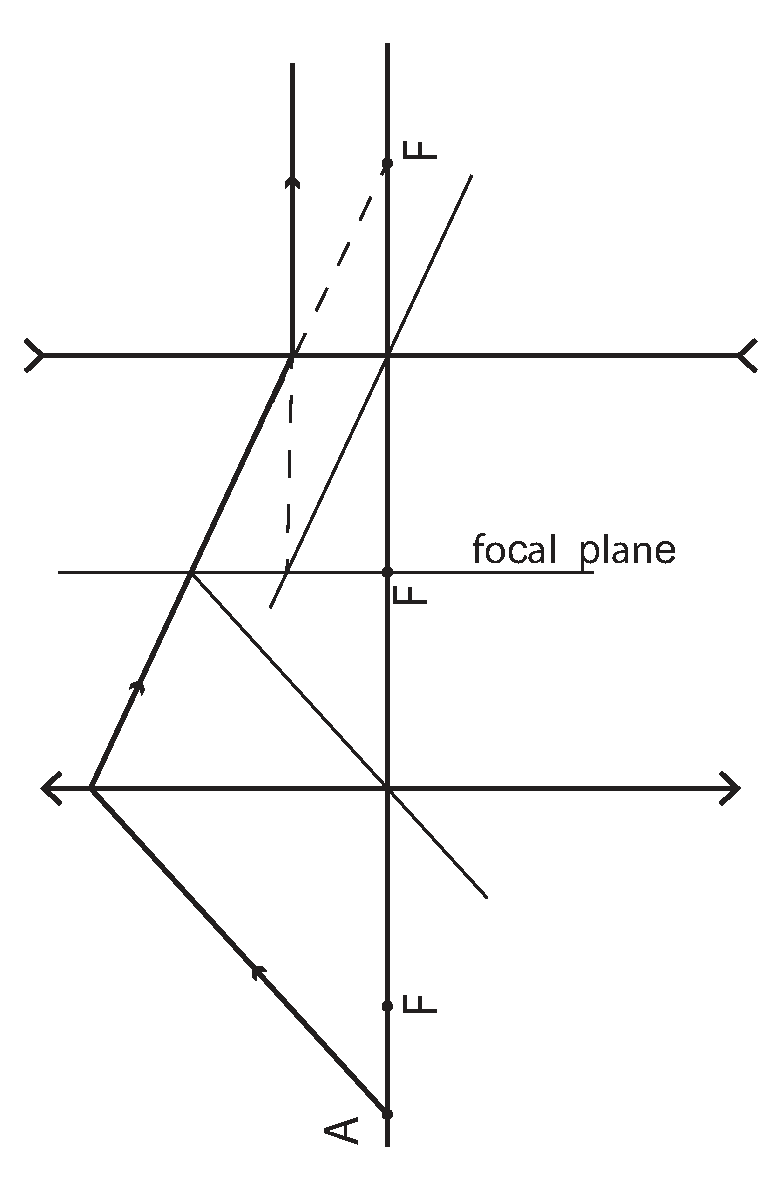
\includegraphics[width=0.7\linewidth]{2017-lahg-02-valgusallikaslah_ing}
\end{center}
\fi
}